\section{Weather Dataset}
Our second data source is hourly NYC weather, retrieved from the Open-Meteo archive API\footnote{\url{https://open-meteo.com/}}.

\subsection{Dataset Structure}

The dataset contains hourly weather observations for New York City, aligned to the \texttt{America/New\_York} timezone. It provides environmental variables used to explain changes in cycling demand.

\subsubsection{Original Structure}

The dataset includes the following main fields:
\begin{itemize}
  \item \textbf{Timestamp}: hourly observation time.
  \item \textbf{Temperature (temperature\_2m)}: air temperature in \si{\degreeCelsius}.
  \item \textbf{Precipitation}: hourly precipitation in millimetres.
  \item \textbf{Weather Code}: WMO weather condition code.
  \item \textbf{Wind Speed (wind\_speed\_10m)}: wind speed in km/h.
  \item \textbf{Year}: derived field used to partition the dataset into annual Parquet files.
\end{itemize}

The dataset is used almost entirely in its original form, with only the \texttt{Year} column added during preprocessing. Weather data are retrieved from the Open-Meteo archive for the same period covered by the trip dataset.

\subsection{Analysis and Insights}
\begin{comment}
    Follows notebook 2.2 "Distributions and Seasonality" and 2.3 "Ridership vs. Weather".
    Per the exam requirements (Deliverable 2 - EDA criterion: "appropriate descriptive
    statistics, visual summaries, and initial insights"), this section should show:
      - Distribution/seasonality plots for temperature and precipitation. Note
        precipitation is zero for most hours with occasional spikes (right-skewed),
        so the histogram should focus on non-zero values.
      - A plot relating ridership to temperature (and/or other weather variables),
        with the insight that ridership rises with temperature up to a comfortable
        range and drops off in the cold - the main justification for including this
        dataset in the project.
\end{comment}

The exploratory analysis focuses on weather distributions and their relationship with ridership.

Temperature follows a clear annual cycle, while precipitation is highly right-skewed: most hours record no rainfall, with occasional heavy events. Consequently, precipitation histograms focus on non-zero observations. Wind speed shows moderate variation throughout the year. Figure~\ref{fig:weather_trends} summarizes the main weather distributions and their seasonal behaviour.

\begin{figure}[ptb]
  \centering
  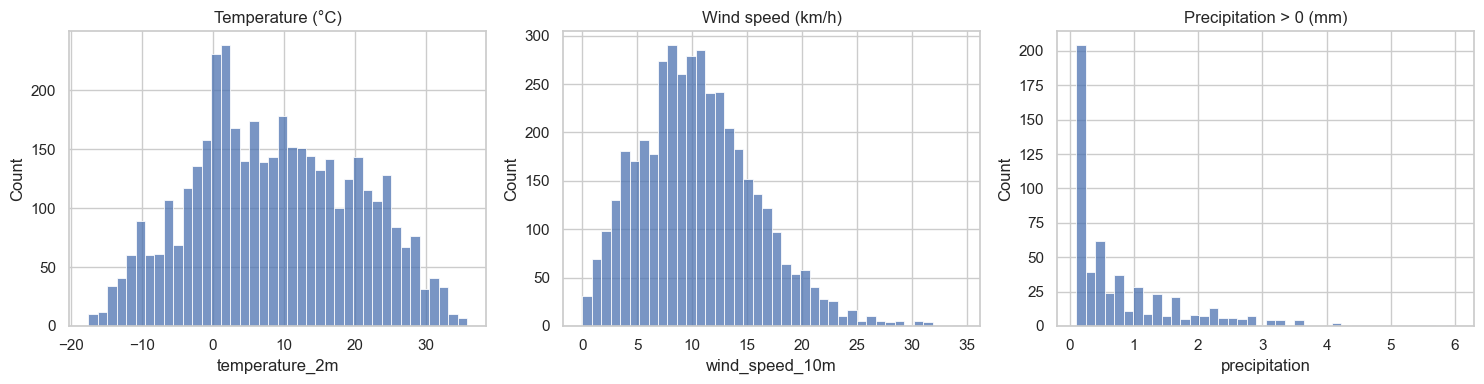
\includegraphics[width=\textwidth]{../media/weather_trends.png}
  \caption{Temperature, wind speed and precipitation distributions over time.}
  \label{fig:weather_trends}
\end{figure}

Hourly trip counts are joined with weather observations using their timestamps. The resulting analysis shows that ridership, as expected, is higher during warmer periods and lower during cold or inclement weather. Two plateaus are observed between \SI{15}{\degreeCelsius} and \SI{20}{\degreeCelsius}, and between \SI{25}{\degreeCelsius} and \SI{30}{\degreeCelsius}. With higher temperatures, ridership increases noticeably, as shown in Figure~\ref{fig:rides_vs_temp}.

\begin{figure}[ptb]
  \centering
  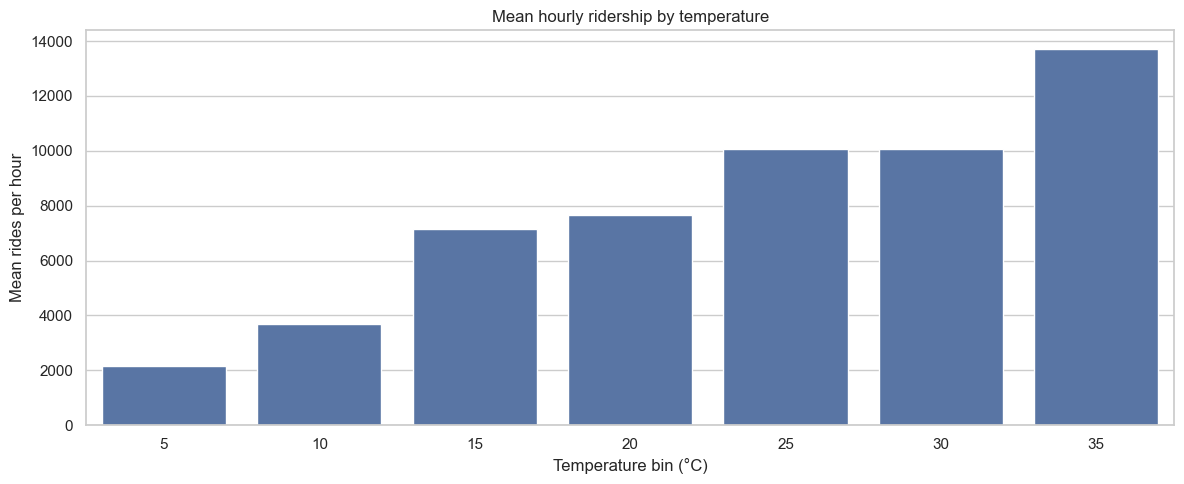
\includegraphics[width=.95\textwidth]{../media/rides_vs_temp.png}
  \caption{Ridership vs.\@ temperature.}
  \label{fig:rides_vs_temp}
\end{figure}

These results justify including weather as an explanatory variable for temporal variations in bike usage.

\subsection{Data Quality}
\begin{comment}
    TODO:
    No missing data, seem to be good quality. Only potential bias is that we use a single 
    weather station (Central Park) to represent all of NYC, but this is a common approach and
    should be fine for our purposes.
\end{comment}

The archived weather data are complete and consistently sampled at hourly intervals, with no significant missing values.

The main limitation is spatial coverage: the dataset represents weather at a single observation location rather than capturing microclimate differences across the five boroughs. While this may introduce some bias, it is a common approximation for city-scale analyses.

Precipitation is strongly skewed, so non-zero values are analysed separately from dry hours. The derived \texttt{Year} column is used only for data partitioning, while additional features such as temperature bins are created only when required for specific analyses.